%versi 2 (8-10-2016) 
\chapter{Pendahuluan}
\label{chap:intro}
   
\section{Latar Belakang}
\label{sec:label}
Project KIRI\footnote{\href{https://projectkiri.id}{https://projectkiri.id}} (akan disingkat sebagai KIRI dalam dokumen ini) adalah sebuah perangkat lunak berbasis web yang dibuat untuk \mbox{membantu} mengurangi efek dari kemacetan. KIRI mengurangi dampak kemacetan dengan membantu penggunanya, baik \mbox{masyarakat} maupun turis, dalam menggunakan salah satu sarana transportasi umum yang ada di Indonesia, yaitu angkutan kota (angkot). Cara KIRI \mbox{mempermudah} penggunaan angkot adalah dengan menunjukkan rute yang akan ditempuh, beserta langkah-langkah yang harus dilakukan oleh pengguna yang ingin berpergian dari satu titik ke titik lain, mulai dari seberapa jauh pengguna harus berjalan untuk menaiki angkot yang bersangkutan, di mana pengguna harus naik atau turun, seberapa jauh lagi pengguna harus berjalan sampai ke titik tujuan, dan seberapa lama estimasi waktu perjalanan yang akan ditempuh. Untuk kebutuhan pembuatan perangkat lunak yang memanfaatkan fitur dari KIRI, tersedia juga REST API KIRI yang dapat digunakan secara praktis. Adapun tampilan dari halaman web ini dapat dilihat di gambar \ref{fig:kiri-page}. 

\begin{figure}[ht]
    \centering
    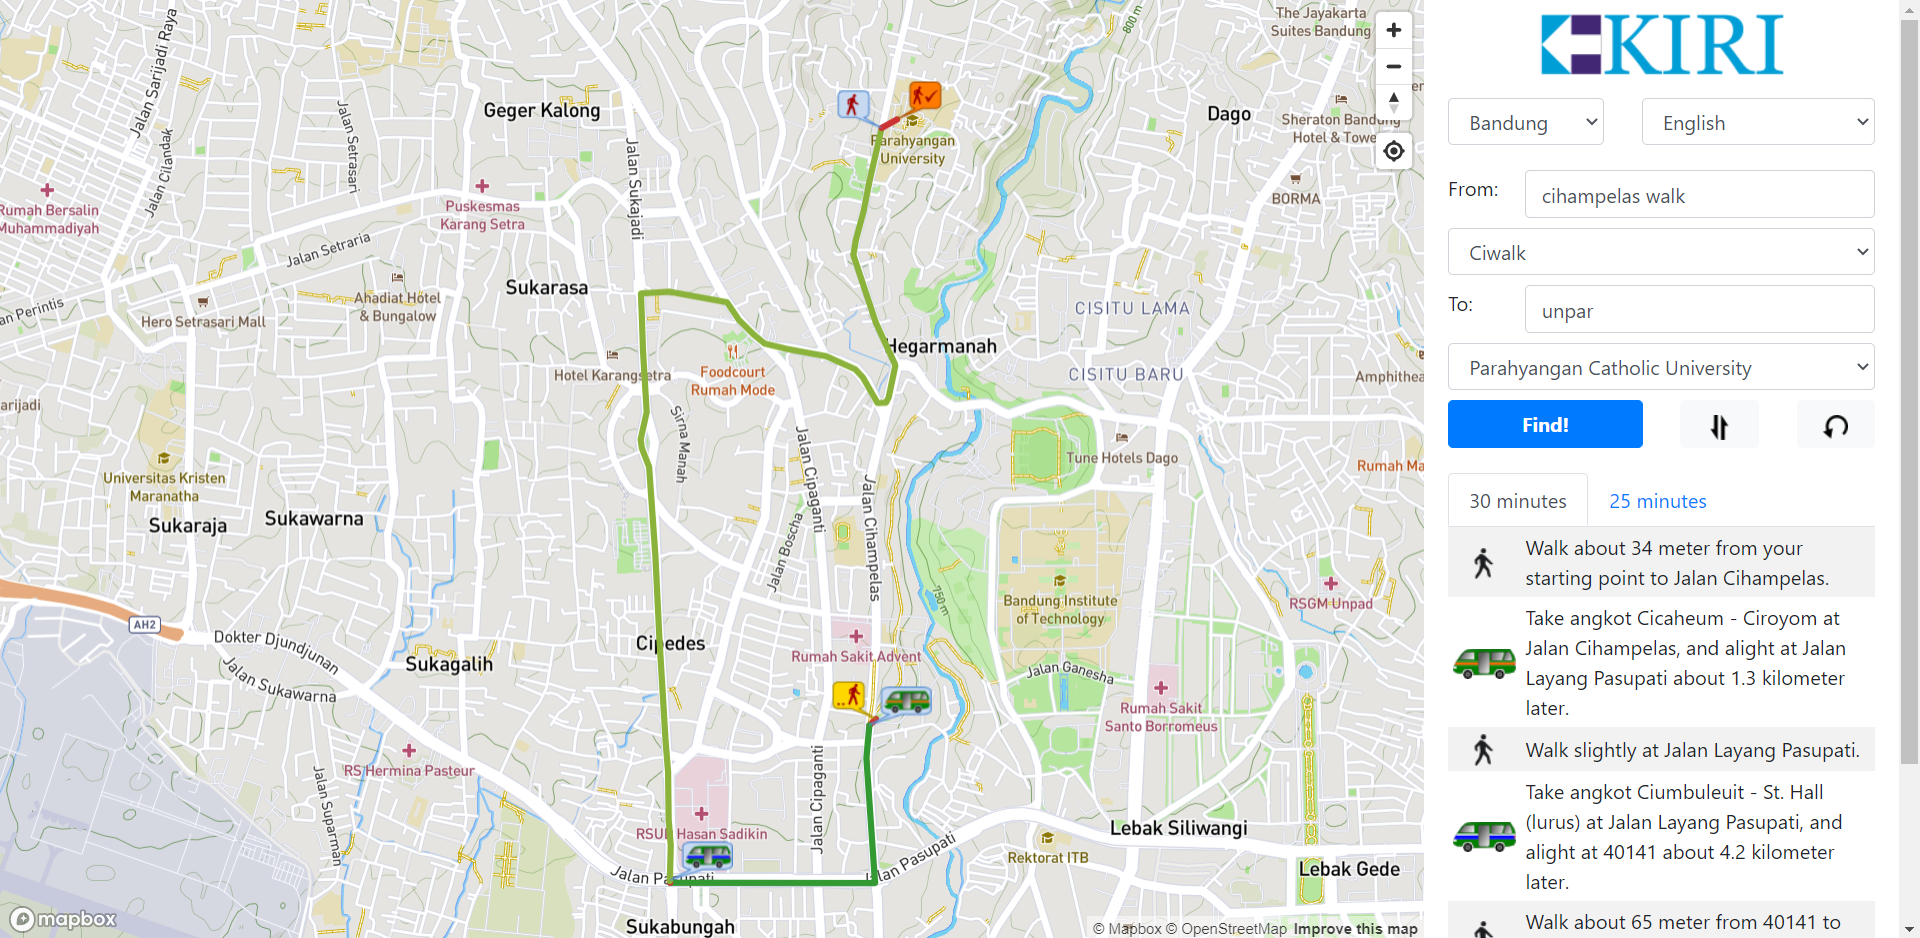
\includegraphics[width=0.74\linewidth]{projectkiri-example}
    \caption[Tampilan halaman web KIRI]{Tampilan halaman web KIRI, yang menunjukkan rute dari Cihampelas Walk ke Universitas Katolik Parahyangan.}
    \label{fig:kiri-page}
\end{figure}

Sementara itu, dalam komputer, salah satu dari sekian banyak tipe perangkat lunak adalah perangkat lunak \textit{command line}. \textit{\mbox{Command} line} (\cl \textit{interpreter}, atau \cl \textit{interface}) adalah sebuah perangkat lunak berupa sebuah kotak/\textit{window} yang memuat teks berupa perintah-perintah,\footnote{\href{https://ubuntu.com/tutorials/command-line-for-beginners\#3-opening-a-terminal}{Ubuntu Tutorials - The Linux command line for beginners: 3. Opening a Terminal}} yang menerima masukan dari pengguna dan  menjalankannya.\cite{marsh:2010:fatfreeintrotocommandline} Perintah-perintah ini hanya berupa gabungan dari teks and simbol-simbol berupa karakter, tanpa ada tambahan gambar grafis apapun. Singkatnya, tipe perangkat lunak ini bukan merupakan tipe yang paling indah untuk dilihat oleh para pengguna, tetapi jika digunakan dengan tepat, maka \mbox{jenis} \mbox{perangkat} lunak ini bisa menyuruh komputer untuk melakukan banyak sekali perintah-perintah dengan sangat cepat dan sangat efektif.

Pada skripsi ini akan dibuat sebuah perangkat lunak berupa perkakas \cl (\textit{command line tool}) yang dapat menjalankan fungsi-fungsi API dari KIRI. Perangkat lunak ini, seperti jenisnya, akan dibuat murni sebagai perkakas yang dijalankan dari \cl (terminal, cmd, PowerShell, dll.), dan tampilan akhir dari perangkat lunak akan berupa \cli tanpa tambahan \textit{graphical user interface}. Keseluruhan dari perangkat lunak ini akan dibangun dalam bahasa C.

\section{Rumusan Masalah}
\label{sec:rumusan}
Rumusan masalah yang akan dibahas dalam skripsi ini adalah sebagai berikut:
\begin{enumerate}
	\item Bagaimana membangun perkakas \textit{command line} yang dapat mengimplementasikan fitur-fitur API KIRI dalam bahasa C?
	\item Bagaimana integrasi perkakas \textit{command line} KIRI dapat dilakukan dengan perkakas-perkakas \textit{command line} lainnya?
\end{enumerate}

\section{Tujuan}
\label{sec:tujuan}
Tujuan dari skripsi ini adalah sebagai berikut:
\begin{enumerate}
	\item Membangun perkakas \textit{command line} yang dapat mengimplementasikan fitur-fitur API KIRI dalam bahasa C.
	\item Melakukan integrasi perkakas \textit{command line} KIRI dengan perkakas-perkakas \textit{command line} lainnya.
\end{enumerate}

\section{Batasan Masalah}
\label{sec:batasan}
Batasan masalah dalam skripsi ini adalah sebagai berikut:
\begin{enumerate}
	\item Perangkat lunak dibuat murni dalam bentuk CLI, tanpa tambahan GUI.
	\item Perangkat lunak yang dibuat tidak menyelesaikan batasan (lokasi tidak terdeteksi, rute tidak berhasil ditemukan, dsb.) yang sudah sejak awal terdapat dalam KIRI.
\end{enumerate}

\section{Metodologi}
\label{sec:metlit}
Metodologi yang akan diikuti dalam skripsi ini adalah sebagai berikut:
	\begin{enumerate}
		\item Melakukan studi dan eksplorasi terhadap fungsi-fungsi yang dimiliki perangkat lunak KIRI serta cara implementasi API KIRI.
		\item Melakukan analisis dan desain perangkat lunak yang akan dibangun.
	    \item Melakukan studi dan eksplorasi terhadap seluruh kemungkinan \textit{library-library} yang memenuhi spesifikasi dalam pembuatan perangkat lunak, berdasarkan analisis dan desain yang telah dilakukan sebelumnya.
		\item Melakukan analisis kebutuhan fitur-fitur perangkat lunak dan melakukan eksplorasi \textit{library} yang dapat digunakan dan memenuhi spesifikasi dalam pembuatan perangkat lunak.
		\item Membangun perangkat lunak berdasarkan rancangan yang sudah dibuat, dengan megimplementasikan seluruh modul dan \textit{library} yang telah ditentukan di tahap sebelumnya dalam bahasa C.
		\item Melakukan pengujian fungsional, perbaikan \textit{bug}, serta rekomendasi perbaikan berdasarkan pengujian yang sudah dilakukan.
		\item Menyelesaikan pembuatan dokumen-dokumen yang berkaitan, seperti dokumen skripsi dan dokumentasi perangkat lunak.
	\end{enumerate}

\section{Sistematika Pembahasan}
\label{sec:sispem}
Setiap bab dalam skripsi ini mengikuti sistematika yang terdiri atas poin-poin sebagai berikut:
\begin{enumerate}
	\item Bab 1: Pendahuluan \\
	Bab ini berisi latar belakang, rumusan masalah, tujuan, batasan masalah, metodologi \mbox{penelitian}, dan sistematika pembahasan.
	\item Bab 2: Dasar Teori \\
	Bab ini berisi pembahasan-pembahasan teoritis mengenai aspek-aspek yang akan dirujuk di dalam skripsi ini, seperti \cl, bahasa C, dan juga KIRI.
	\item Bab 3: Analisis \\
	Bab ini berisi analisis perkakas-perkakas sejenis, analisis API KIRI, serta analisis kebutuhan perkakas yang akan dibuat.
	\item Bab 4: Perancangan \\
	Bab ini berisi pembahasan mengenai rancangan cara kerja tiap-tiap fitur perkakas yang akan dibuat.
	\item Bab 5: Implementasi dan Pengujian \\
	Bab ini berisi dua bagian utama, yaitu:
	
	\begin{itemize}
		\item Implementasi \\
		Bagian ini meliputi struktur kelas dan penjelasan tiap-tiap fungsi di dalamnya.
		\item Pengujian \\
		Bagian ini meliputi cara instalasi, cara menggunakan perkakas, serta pengujian fungsional terhadap fitur-fitur dari perkakas yang telah dibuat. dalamnya.
	\end{itemize}
	
	\item Bab 6: Kesimpulan dan Saran \\
	Bab ini berisi kesimpulan hasil pembuatan perangkat lunak dan saran-saran terhadap hasil perangkat lunak yang diberikan selama pengerjaan skripsi.
\end{enumerate}